How to use the same key for symmetric encryptions?
How to obtain the public key of others?
We can solve this by building cryptographic protocols.

\subsection{Key Management}
Remember Kerckhoff's principle: the security of a cryptosystem should not depend on the secrecy of the algorithm, but only on the secrecy of the key.

Using the right cryptographic algorithms, the problem of protecting
data is transferred to the problem of protecting keys.
Key management is the backbone of cryptography. \\

Key management includes:
\begin{itemize}
    \item Key Generation
    \item Key Distribution
    \item Key Storage
    \item Key Usage
    \item Key Destruction
\end{itemize}

\subsubsection{Key Generation}
Requirements:
\begin{itemize}
    \item Secret
    \item Unpredictable
    \item Strong key
\end{itemize}

Methods:
\begin{itemize}
    \item Manual (tossing):  without automated tools or systems, often using simple physical or manual techniques
    \item (Pseudo) Random Number Generators (FSR)
\end{itemize}

Secure hardware, secure room, and secure procedures are needed!

\subsubsection{Key Freshness}
It is often desirable to frequently change the key in a cryptographic
system. This is called \textbf{key freshness}.

\begin{itemize}
    \item If a key is exposed (e.g., through hackers), there is limited
    damage if the key is changed often
    \item Some cryptographic attacks become more difficult if only a
    limited amount of ciphertext was generated under one key
    \item If an attacker wants to recover long pieces of ciphertext, he has
    to recover several keys which makes attacks harder
\end{itemize}

\subsubsection{Types of Keys and Key Distribution}
\begin{itemize}
    \item \textbf{Static Key}: used for a long time (long-term, few hours to years)
    \item \textbf{Session/Ephemeral Key}: used for a single session or a limited time (short-term, a few seconds or a day)
    \item \textbf{Master Key}: used to generate session keys
\end{itemize}

Key distribution is the process of securely delivering keys to the parties that need them. Done through:
\begin{itemize}
    \item Physical distribution
    \item Distribution using symmetric key protocols 
    \begin{itemize}
        \item Distributing this key securely over an untrusted channel is difficult, as an attacker could intercept it
    \end{itemize}
    \item Distribution using public (asymmetric) key protocols
    \begin{itemize}
        \item While public keys can be shared openly, ensuring the authenticity of a public key (i.e., that it belongs to the claimed entity) is a key distribution problem
    \end{itemize}
\end{itemize}

\subsection{Key Distribution Problem}
The \textbf{key distribution problem} refers to the challenge of securely sharing cryptographic keys between parties in a way that prevents unauthorized access or interception. 
This issue is fundamental in cryptography because the security of encrypted communication depends on the secrecy of the key. \\

\textbf{Example:} In a symmetric key system, the number of unique keys required for secure communication
between $n$ participants is given by:

\[ \frac{n(n-1)}{2}\]

This formula accounts for every pair of participants needing a unique key to securely communicate.
 every student would need to share a unique private key with every other student in order to securely communicate.
Say TU Delft has $n=250000$ students, then the number of keys required is:

\[ \frac{250000(250000-1)}{2} = 31,249,875,000 \]

in a \emph{symmetric key system}. Every student would need to share a unique private key with every other student in order to securely communicate! This is clearly infeasible.
Also, what if your key is compromised: what can you do? And what can the attacker do? (decrypt past communications, impersonate the legitimate user)

\subsection{Certificates and Certiface Authorities}
Say Alice and Bob share a symmetric key. We assume they have a \textbf{shared, long-term (secret) key} $K_{ab}$.
This key must be distributed via a secure channel = courier. \\

In the case that they use assymetric keys, Alice has Bob's public key and Bob has Alice's public key.
How can either of them be shure that the public key they have is actually Bob's or Alice's?
This is where \textbf{certificates} come in. \\

In \textbf{binding}, a public key is linked to an entity. Some examples of this are:
\begin{itemize}
    \item Physical tokens such as smart cards (PIN number, biometrics)
    \item Digital certificates
\end{itemize}

\begin{defn}
    A \textbf{certificate} in cryptography is a digital document used to prove the authenticity of a public key. It contains the following:

    \begin{itemize}
        \item \textbf{Public Key}: The key associated with a user, system, or entity.
        \item \textbf{Identity Information}: Information about the owner, such as their name or organization.
        \item \textbf{Signature}: A digital signature from a trusted authority (like a Certificate Authority, or CA) to validate that the certificate and its contents are legitimate.
        \item \textbf{Name of the CA}
        \item \textbf{Serial number of the certificate}
        \item \textbf{Expiry data of the certificate}

    \end{itemize}
    
    Certificates are widely used in \textbf{Public Key Infrastructure (PKI)} to ensure secure communication by verifying the identity of the public key holder. They help prevent impersonation and man-in-the-middle attacks.     
\end{defn}

\begin{defn}
    A \textbf{Certificate Authority} (CA) is a trusted organization or entity that issues digital certificates. 
    Also called \textbf{Trusted Third Party (TTP)}. \\

    These certificates verify the identity of entities (such as websites, organizations, or individuals) and link them to their public keys. 
    The CA ensures that the public key belongs to the entity it claims to represent by digitally signing the certificate. 
    This process helps establish trust in secure communications, such as in \emph{SSL/TLS} connections, by preventing impersonation and ensuring data integrity.

    \begin{itemize}
        \item All users have a copy of the CA's public key
        \item CA signs the data string (Alice, Alice's public key). This is the certificate.
        \item Alice sends people her public key and the certificate
    \end{itemize}
\end{defn}

\subsubsection{Certificate Chain}
A \textbf{certificate chain} is a sequence of digital certificates used to establish trust between a user's certificate and a trusted root certificate. It typically includes:

\begin{itemize}
    \item \textbf{End-entity Certificate}: The certificate of the user or website.
    \item \textbf{Intermediate Certificates}: Certificates issued by intermediate Certificate Authorities (CAs) that bridge the gap between the end-entity certificate and the root certificate.
    \item \textbf{Root Certificate}: The self-signed certificate of a trusted CA that anchors the trust chain.
\end{itemize}

The certificate chain ensures that the end-entity certificate is trusted by tracing back to a trusted root certificate, helping verify the authenticity and integrity of the certificate.

\begin{figure}[h!]
    \centering
    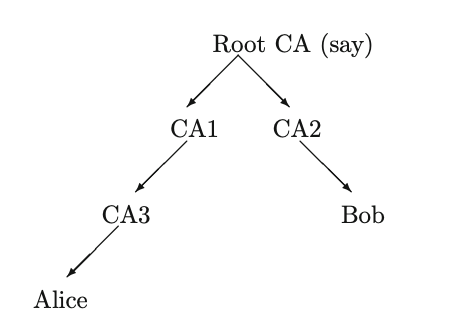
\includegraphics[width=0.25\textwidth]{img/cchain.png}
    \caption{Certificate Chain}
\end{figure}

The task of the CA is to verify the identity of the entity and to sign the certificate. Usually split up into two:

\begin{itemize}
    \item \textbf{Registration Authority (RA)}: verifies the identity of the entity (personal data), accepts, registers: contact with the client
    \item \textbf{Certificate Authority (CA)}: generation, management, and distribution of PK-certificates
\end{itemize}

\subsubsection{Certificate Revocation}
Say that the key is compromised. Then a previously issued digital certificate must be invalidated before its expiration date.
Can happen if:
\begin{itemize}
    \item The private key associated with the certificate is compromised
    \item The certificate holder's information changes or is no longer valid
    \item The certificate was issued incorrectly or fraudulently
\end{itemize}

Everybody should be warned of this. This is done through \textbf{Certificate Revocation Lists (CRLs)} or \textbf{Online Certificate Status Protocol (OCSP)}.
They allow users and systems to check the \emph{status of a certificate} and verify if it has been revoked. \\

The system of CAs and certificates is called \textbf{Public Key Infrastructure (PKI)}.

\subsubsection{Implicit Certificates}
Typical certificates can be quite large. We can also have a smaller certificate that binds the 
public keu and the data in the form of $X|Y$, where:

\begin{itemize}
    \item $X$ is the data being bound to the public key
    \item $Y$ is the implicit certificate on $X$
\end{itemize}

From $Y$ we can obtain the public key bound to $X$. Implicit certificates do not \emph{explicitly} contain the identity
information of the certificate holder.\\

For example, in some systems, the certificate may only include a public key and be automatically associated with a specific entity based
on the environment or protocol in use. These certificates rely on pre-existing trust relationships or predefined roles,  
rather than explicitly storing detailed identity information within the certificate itself. \\


\Comment{I dont understand this protocol...}
\textbf{Protocol:}
\begin{enumerate}
    \item System setup: the CA chooses a public group $G$ of order $n$, and an element $P$. 
    The private key is $x$, the public key is $P^x$.

    \item Certificate request: the ephemeral key is $t$, shared between the CA and the user. User has ID. 
    The public key is $R=P^t$. The user sends the ID and the public key to the CA.

    \item Processing of the request: the CA picks another random $k$, and computes:
    \begin{itemize}
        \item $g \leftarrow P^kR = P^kP^t = P^{k+t}$
        
        \item $s \leftarrow x H(ID||g) + k \pmod{n}$
        
        \item CA sends $(g,s)$ to the user
    \end{itemize}


    \item User's key discovery: from $t, s, R = P^t$, the key is $P^{\text{user}} = P^{t+s} = P^tP^s = R \cdot P^s$ \\
    $P^{\text{user}} = Q^{H(ID||g)}g$

\end{enumerate}

Problems: CA is compromised, has the same level security with the users, not good.

\subsection{Key Agreement protocols}

\textbf{Key agreement} allows two or more parties to securely agree on a shared secret key, 
which can be used for encrypted communication. 
The key is established without directly transmitting it over an insecure channel.

\subsubsection{Symmetric Key Agreement}
In key agreement schemes that use static symmetric keys to derive ephemeral keys, 
the parties exchange information to derive a new, session-specific ephemeral key. 
The static key might be used to help authenticate the participants or securely exchange the ephemeral key information. \\

This approach ensures \textbf{forward secrecy}, meaning that past sessions remain secure even if long-term keys are compromised.
Also, better security for each session by using new keys for each interaction. A compromise on key should not lead to security problem on the
previous messages decrypted before that time. \\

The number of keys is $n(n-1)/2$. Short term keys are derived from long-term keys, using symmetric systems. Some definitions:

\begin{itemize}
    \item Parties: A, B, and TTP
    \item Shared keys: $K_{ab}, K_{bs}, K_{As}$
    \item Nonces: numbers used \textbf{only once}, unique but not necessarily random (to prevent replay attacks)
    \item Timestamps: time of the message $T_a, T_b$
\end{itemize}

\[ A \rightarrow B: M, A, B, \{N_a, M, A, B\}_{K_{as}}\]

where:
\begin{itemize}
    \item $A \rightarrow B$: Party A is sending a message to Party B
    \item $M$: some message or data that Party A wants to send to Party B
    \item $\{N_a, M, A, B\}_{K_{as}}$: This is an encrypted part of the message. Specifically:
    \begin{itemize}
        \item $N_a$: A nonce generated by Party A
        \item $M$: The original message that Party A wants to send.
        \item $A, B$: The identities of the sender and receiver, A and B, included in the encrypted portion to authenticate the message.
        \item $\{\cdots \}_{K_{as}}$: This denotes that the contents inside the braces (the nonce, message, and party identifiers) 
        are encrypted using the shared symmetric key $K_{as}$ between Party A and the TTP (Trusted Third Party, denoted by ``S" in this case).
    \end{itemize}
\end{itemize}

\subsubsection{Wide-Mouth Frog Protocol}
The Wide-Mouth Frog Protocol is a key agreement protocol based on a TTP where a ``frog" (a participant)
communicates with a trusted intermediary to establish a shared secret with another party.

\begin{figure}[h!]
    \centering
    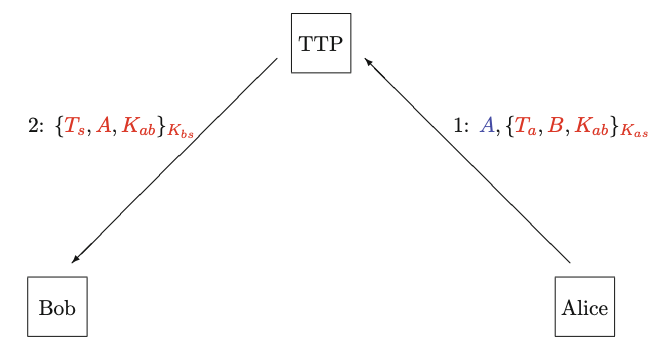
\includegraphics[width=0.4\textwidth]{img/frog.png}
    \caption{Wide-Mouth Frog Protocol}
\end{figure}

Simple, but has issues:
\begin{itemize}
    \item Reliance on TTP: if TTP is compromised, security of entire system is compromsed. TTP handles all key exhanges.
    \item No authentication of parties involved in the key exchange. Attacker can impersonate a party (man-in-the-middle attack)
    \item No nonces, timestamps, or other mechanisms to prevent replay attacks
    \item No forward secrecy: if long-term key is compromised, all past sessions are compromised
    \item TTP is a \textbf{single point of attack}
\end{itemize}

\subsubsection{Man-in-the-Middle Attack}
$E$ is the attacker/intermediary. $S$ is the trusted third party.

% \begin{equation}
%     \begin{aligned}
%         A &\rightarrow E: A,B \\
%         E &\rightarrow S: A,E \\
%         S &\rightarrow E: K_{ae_{K_{es}}}, K_{ae_{K_{as}}}  \\
%         E &\rightarrow A: K_{ae_{K_{es}}}, K_{ae_{K_{as}}} \\
%         A &\rightarrow E: K_{ae_{K_{as}}}, A
%     \end{aligned}
% \end{equation}

\begin{align*}
    A &\rightarrow E: A, B \\
\end{align*}
\textbf{Step 1:} 
\begin{itemize}
    \item Party \textbf{A} sends a message to \textbf{E} with information identifying \textbf{A} and \textbf{B}.
\end{itemize}

\begin{align*}
    E &\rightarrow S: A, E \\
\end{align*}
\textbf{Step 2:} 
\begin{itemize}
    \item The attacker \textbf{E} forwards the message to \textbf{S}, but with \textbf{E}'s own identity instead of \textbf{B}'s.
    \item This tricks \textbf{S} into thinking that \textbf{A} is trying to establish a connection with \textbf{E}.
\end{itemize}

\begin{align*}
    S &\rightarrow E: K_{ae_{K_{es}}}, K_{ae_{K_{as}}} \\
\end{align*}
\textbf{Step 3:}
\begin{itemize}
    \item The server \textbf{S} responds to \textbf{E}, sending two keys:
    \begin{itemize}
        \item $K_{ae_{K_{es}}}$: Key for \textbf{A} encrypted with a shared key between \textbf{E} and \textbf{S}.
        \item $K_{ae_{K_{as}}}$: Another key for \textbf{A} encrypted with a different shared key.
    \end{itemize}
    \item \textbf{S} is unaware that \textbf{E} is an attacker.
\end{itemize}

\begin{align*}
    E &\rightarrow A: K_{ae_{K_{es}}}, K_{ae_{K_{as}}} \\
\end{align*}
\textbf{Step 4:}
\begin{itemize}
    \item The attacker \textbf{E} forwards the keys it received from \textbf{S} to \textbf{A}.
    \item \textbf{A} assumes the keys were sent by \textbf{S}, but they were actually manipulated by \textbf{E}.
\end{itemize}

\begin{align*}
    A &\rightarrow E: K_{ae_{K_{as}}}, A \\
\end{align*}
\textbf{Step 5:}
\begin{itemize}
    \item Party \textbf{A} sends a confirmation message back to \textbf{E}, verifying the keys and identifying itself.
    \item \textbf{A} believes it is still securely communicating with \textbf{S}, but \textbf{E} has positioned itself as an intermediary.
\end{itemize}

\begin{figure}[h!]
    \centering
    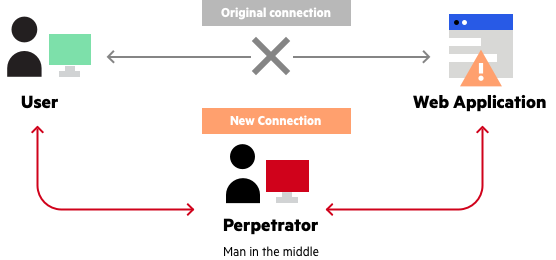
\includegraphics[width=0.4\textwidth]{img/mitm.png}
    \caption{Man-in-the-Middle Attack}
\end{figure}

Outcome: \textbf{E} now has the keys intended for \textbf{A} and can decrypt, read, or modify messages between \textbf{A} and \textbf{S}. 
\textbf{A} believes it is directly communicating with \textbf{S}, and \textbf{S} believes it is communicating with \textbf{A}, but in reality, \textbf{E} is in the middle, manipulating the communication.

\subsubsection{Needham-Schroeder Protocol}
The \textbf{Needham-Schroeder Protocol} is an authentication protocol designed to securely establish
secure communication between parties. Aims to prevent attacks like MITM by using timestamps and nonces in its message exchanges. 

\begin{enumerate}
    \item $A$ sends a request to TTP to request a session key to communicate with $B$.
    \item TTP responds with two parts:
    \begin{itemize}
        \item An encrypted version of the session key $K_{ab}$, encrypted wth $A$'s shared key with TTP. Only $A$ can decrypt this part.
        \item An encrypted version of the session key $K_{ab}$ (along with $A$'s identity), encrypted with $B$'s shared key with TTP, $K_{bs}$. Only $B$ can decrypt this part.
    \end{itemize}

    \item $A$ forwards the second part of the message to $B$: $A \leftarrow B : \{K_{ab}, A\}_{K_{bs}}$
    \item $B$ decrypts the message, retrieves the session key $K_{ab}$, and sends a confirmation back to $A$ using its nonce.
    \item $A$ decrypts the confirmation message, retrieves the nonce, and sends a confirmation back to $B$ using the nonce (minus 1).
\end{enumerate}


\begin{figure}[h!]
    \centering
    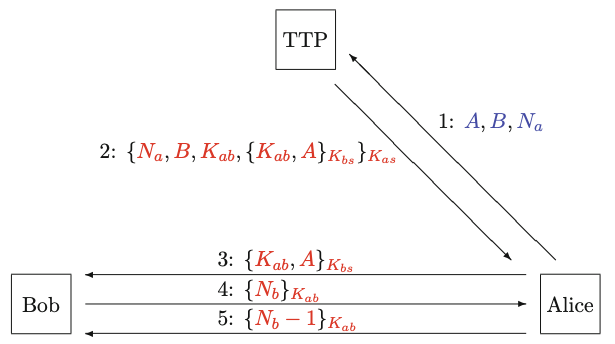
\includegraphics[width=0.5\textwidth]{img/needham.png}
    \caption{Needham-Schroeder Protocol}
\end{figure}

This protocol prevents MITM attacks through:
\begin{itemize}
    \item Nonces
    \item Encryption of messages with shared keys
    \item Session key exchange
    \item Authenticated communication
    \item Prevents replay attacks
\end{itemize}

Remember: A \textbf{replay attack} occurs when an attacker intercepts a valid message between two parties and then replays (or resends) it later,
in an attempt to make it appear as a legitimate request.
Without any protection, this would allow attackers to trick the system into accepting the intercepted message, as it looks like a valid communication. \\

By using nonces, each message is unique and fresh. If the nonce in the message does not match the one expected by the recipient, the message is rejected. \\

\textbf{Kerberos} is an authentication system based on symmetric encryption, building on the Needham-Schroeder protocol.
Difference is that Kerberos uses timestamps. This does require \emph{synchronized clocks} between parties. \\

To summarize, symmetric key systems deal with the key distribution problem. TTP based solutions like Kerberos are also problemaitc, because
they assyme that there is a long-term key. Two techniques that solve this problem:
Key transport based on public key cryptography, and key agreement that outputs a symmetric key.

\subsubsection{Assymetric Key Agreement}
All schemes up to now are not forward secure! Once compromised, all messages in the past can be decrypted.
\textbf{Asymmetric Key Agreement} is a process where two parties use public-key cryptography to establish a shared secret key over an insecure channel. \\

\textbf{Steps:}
\begin{enumerate}
    \item \textbf{Key Pair Generation}: Each party generates a pair of keys (public, secret).
    
    \item \textbf{Exchange of Public Keys}: The parties exchange their \textbf{public keys} over an insecure channel.
    
    \item \textbf{Computation of Shared Secret}: Each party uses their \textbf{private key} and the other party's \textbf{public key} to compute the same \textbf{shared secret key}.
    
    \item \textbf{Symmetric Encryption}: Once the shared secret is established, both parties can use it for symmetric encryption to secure further communication.
\end{enumerate}

No prior shared secret is needed. The shared secret is used for symmetric encryption after exchange.

\subsubsection{Diffie-Hellman Key Exchange Protocol}
Enables two entities to establish a symmetric key even though they have never met before. Based on the \textbf{discrete log problem}. \\

Finding the exponent \( x \) in the equation:
\[
g^x \equiv y \ (\text{mod} \ p)
\]

For large values of \( p \) and \( g \), this is computationally infeasible. 
Finite field version on Abelian group $G$ of order $p$. There is also an elliptic curve version. \\

In Diffie-Hellman, the parties use a publicly known base and modulus, but each party generates their own private key.

\begin{figure}[h!]
    \centering
    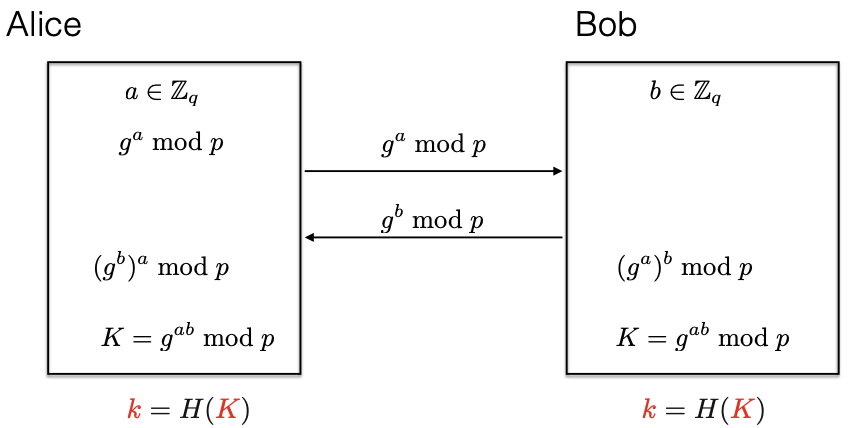
\includegraphics[width=0.5\textwidth]{img/DHkeyprotocol.png}
    \caption{Diffie-Hellman Key Exchange Protocol}
\end{figure}

Because this protocol in its basic form does not authenticate the identities of the communicating parties, the MITM attack is possible.
There is \textbf{no identity verification for the exhanged public keys}:
\begin{enumerate}
    \item Alice sends her public key to Bob.
    \item Attacker \textbf{E} intercepts Alice's public key and sends their own public key to Bob.
    \item Bob sends his public key to Alice.
    \item Attacker \textbf{E} intercepts Bob's public key and sends their own public key to Alice.
    \item Now, Alice and Attacker \textbf{E} will compute a shared secret using Alice's private key and \textbf{E}'s public key.
    \item Similarly, Bob and Attacker \textbf{E} will compute a shared secret using Bob's private key and \textbf{E}'s public key.
\end{enumerate}
As a result, Attacker \textbf{E} has established two separate shared secrets with each party, allowing them to decrypt, read, and manipulate the messages between Alice and Bob. \\

Solution is \textbf{Signed Diffie-Hellman}: each party can sign their public key with their private key to prove their identity.

\begin{figure}[h!]
    \centering
    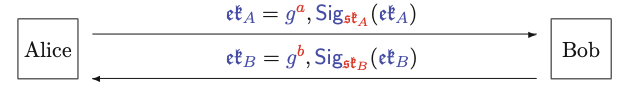
\includegraphics[width=0.5\textwidth]{img/signedDH.png}
    \caption{Signed Diffie-Hellman Key Exchange Protocol}
\end{figure}

However, still not secure because:
\begin{itemize}
    \item Lack of freshness: attacker could reuse an old, signed key from a previous session and trick the system into establishing an insecure connection
    \item Key substiution attack: without certificas/TTP, an attacker can substitute one party’s public key with their own key
\end{itemize}

\subsubsection{Station-to-Station Protocol}
The \textbf{Station-to-Station Protocol} is an extension of the Diffie-Hellman key exchange protocol that adds authentication to the 
key exchange process. Mutual key and entity authentication. Protocol assumes that
parties have signature keys, which are used to sign the messages.
No timestaps. Provides \textbf{perfect forward secrecy}.

\begin{align*}
    &A \rightarrow B: g^x\\
    &B \rightarrow A: g^y, E_K(S_B(g^y, g^x))\\
    &A \rightarrow B: E_K(S_A(g^x, g^y))
\end{align*}

where $g$ is a generator, $x, y$ are private keys of Alice and Bob, respectively.
$S_A, S_B$ are the signatures of $A$ and $B$, and $E_K$ is the encryption with the public key, derived from the shared secret. The steps written out fully are:

\begin{itemize}
    \item Alice generates a random number \( x \) and computes \( g^x \), then sends \( g^x \) to Bob.
    \item Bob generates a random number \( y \) and computes \( g^y \), then computes the shared secret key \( K = (g^x)^y \).
    \item Bob concatenates the exponentials \( (g^y, g^x) \) (order is important), signs them using his private key \( B \), and encrypts the signature with the key \( K \). He then sends the ciphertext along with \( g^y \) to Alice.
    \item Alice computes the shared secret key \( K = (g^y)^x \).
    \item Alice decrypts the ciphertext and verifies Bob's signature using Bob's public key.
    \item Alice concatenates the exponentials \( (g^x, g^y) \) (order is important), signs them using her private key \( A \), and encrypts the signature with the key \( K \). She then sends the ciphertext to Bob.
    \item Bob decrypts and verifies Alice's signature using her public key.
\end{itemize}

A variant with MACs exists.

\subsubsection{MQV Protocol}
Authentication without signatures and MACs. It enhances the Diffie-Hellman method by integrating public key signatures. 
Here, both parties have a long-term key $(g^a, a), (g^b, b)$.
They obtain each others public key via certificates:

\begin{align*}
    &A \rightarrow B: g^x\\
    &B \rightarrow A: g^y
\end{align*}

where $x,y$ are the private keys of Alice and Bob. \Comment{is this true?}
